\documentclass{beamer}
%
% Choose how your presentation looks.
%
% For more themes, color themes and font themes, see:
% http://deic.uab.es/~iblanes/beamer_gallery/index_by_theme.html
%
\mode<presentation>
{
  \usetheme{Warsaw}      % or try Darmstadt, Madrid, Warsaw, ...
  \usecolortheme{default} % or try albatross, beaver, crane, ...
  \usefonttheme{default}  % or try serif, structurebold, ...
  \setbeamertemplate{navigation symbols}{}
  \setbeamertemplate{caption}[numbered]
} 

\usepackage[english]{babel}
\usepackage[utf8x]{inputenc}
\usepackage{graphicx}
\usepackage[ELEC]{aaltologo}
%\usepackage{animate}

\title[ZigBee]{Alternative Network Architectures: ZigBee}
\author{Riku Lääkkölä \and Tero Marttila \and Tero Paloheimo}
\institute{Aalto ELEC}
\date{25.3.2014}
\logo{\AaltoLogoRandomSmall{0.3}}

\begin{document}

\begin{frame}
  	\titlepage
\end{frame}

% Uncomment these lines for an automatically generated outline.
%\begin{frame}{Outline}
%  \tableofcontents
%\end{frame}

\begin{frame}{Introduction}
  \begin{itemize}
    \item ZigBee specifies high-level communication protocols over IEEE 802.15 LR-WPAN.
    \item Used for e.g. home automation, sensor networks?
  \end{itemize}
\end{frame}

\begin{frame}{IEEE 802.15}
  \begin{itemize}
  	\item IEEE 802.15.4
  	\item Low-Rate Wireless Personal Access Networks
	\item Defines Physical and Link layers
  	
    % ZigBee ISA100.11a WirelessHART.
  \end{itemize}
\end{frame}

\begin{frame}{IEEE 802.15 Physical Layer}
  \begin{itemize}
  	\item Provides low-bandwidth transmissions
  	\begin{itemize}
  		\item 868/915 MHz @ 20kbps and 2.4 GHz @ 250kbps
  	\end{itemize}
  	\item Optimized for cheap, low-power hardware
  	\begin{itemize}
    	\item Wakeup from sleep in 30ms (ZigBee)
  	\end{itemize}
  \end{itemize}
\end{frame}
    
\begin{frame}{IEEE 802.15 Link Layer}
  \begin{itemize}
    % CSMA, beacons.
    \item Full-function vs Reduced-function devices
	\begin{itemize}
  		\item Battery-powered devices wake up from sleep to transmit
  		\item Less power-constrained devices can receive continuously
	\end{itemize}
	
  	%\item Addressing (?)
  	%\item Frame validation, time slot guarantees, node assocations.
  	\item Devices form assocations and may relay data
  	\item Coordinator nodes
  \end{itemize}
\end{frame}

\begin{frame}{ZigBee Network Layer}
  \begin{figure}
  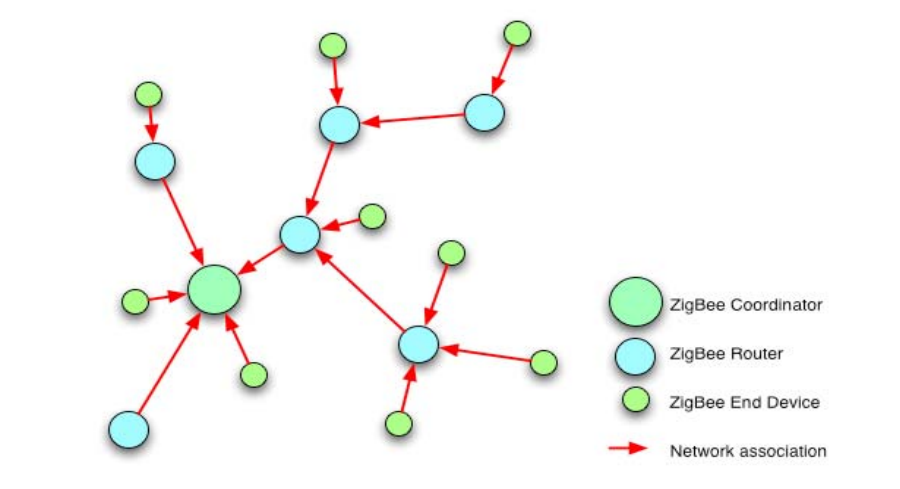
\includegraphics[width=\textwidth]{zbnetstructure.png}
  \caption{ZigBee network structure. Controllers and routers act as IEEE 802.15.4 FFDs and end devices as RFDs.}
  \end{figure}
  \begin{itemize}
  	\item Support for various network structures
  	\begin{itemize}
  		\item Star, Tree, Mesh
  	\end{itemize}
  	\item AODV routing (broadcast request -> unicast response)
  	\item Device types
  	\begin{itemize}
  		\item ZigBee Coordinator
  		\item ZigBee Router
  		\item ZigBee End Device
  	\end{itemize}
  \end{itemize}
\end{frame}

\begin{frame}{ZigBee Application Layer}
  \begin{itemize}
  	\item ZigBee Device Object
  	\begin{itemize}
  		\item Discovery
  		\item Service addressing
  		\item Security
  		\item Configuration (?)
  	\end{itemize}
  	\item Application profiles
  	\begin{itemize}
  		\item Define application-specific protocols 
  	\end{itemize}
  \end{itemize}
\end{frame}

\begin{frame}{ZigBee Application Profiles}
  \begin{itemize}
  	\item ZigBee Home Automation
    \item ZigBee Smart Energy
    \item ZigBee Telecommunication Services
    \item ZigBee Health Care
    \item ZigBee RF4CE – Remote Control
    \item ZigBee RF4CE – Input Device
    \item ZigBee Light Link
    \item ZigBee IP
    \item ZigBee Building Automation
    \item ZigBee Gateway
    \item ZigBee Green Power
  \end{itemize}
\end{frame}

\begin{frame}{IEEE 802.15.4 architecture (continued)}
  \begin{itemize}
    \item Node types  
      \begin{itemize}
      \item Fully-functioning device (FFD) may act as a coordinator in addition
      to being a common node. 
      \item Reduced-function devices (RFD) are simple and may only communicate
      with FFDs.
    \end{itemize}
    \item Network topologies: peer-to-peer and star.
  \end{itemize}
\end{frame}

\begin{frame}{IEEE 802.15.4 Data Transport}
  \begin{itemize}
    \item Basic data transport unit is a frame having four types: data, 
    acknowledgement, beacon and MAC command.
    \item Contention resolved by CSMA/CA.
  \end{itemize}
\end{frame}

\end{document}
